\documentclass[a4paper]{ctexrep}
\usepackage[colorlinks,linkcolor=black]{hyperref}
\usepackage{listings, geometry, amsmath}
\usepackage[colorinlistoftodos]{todonotes}
\usepackage{graphicx}
\usepackage{varwidth}
\usepackage{float}
%\setmonofont[Mapping={}]{Monaco}	%英文引号之类的正常显示,相当于设置英文字体
\definecolor{mygreen}{rgb}{0,0.6,0}
\definecolor{mygray}{rgb}{0.5,0.5,0.5}
\definecolor{mymauve}{rgb}{0.58,0,0.82}
% 代码块设置
\lstset{ % 代码高亮
	backgroundcolor=\color{white},   % choose the background color
	basicstyle=\footnotesize\ttfamily,        % size of fonts used for the code
	columns=fullflexible,
	numbers=left,                    % where to put the line-numbers; possible values are (none, left, right)
	numbersep=0.5em,		% how far the line-numbers are from the code
	breaklines=true,                 % automatic line breaking only at whitespace
	captionpos=t,                    % sets the caption-position to bottom
	tabsize=4,
	frame = single,
	framexleftmargin=2em,
	commentstyle=\color{mygreen},    % comment style
	escapeinside={\%*}{*)},          % if you want to add LaTeX within your code
	keywordstyle=\color{blue},       % keyword style
	stringstyle=\color{mymauve}\ttfamily,     % string literal style
	rulecolor=\color{black},
	% identifierstyle=\color{red},
	language=c++,
	showtabs = false,
	showstringspaces = false,
	showspaces = false,
}

\geometry{left=3cm,right=3cm,top=3cm,bottom=3cm}

\hypersetup{
	pdftitle={实验报告模板},
	pdfauthor={刘朝洋},
	pdfsubject={实验报告模版},
	pdfkeywords={模版},
}

\ctexset {
	chapter = {
		name = {实验, },
	},
	section = {
		number = \arabic{section},
		format = \Large\bfseries,
	},
	subsection = {
		number = \arabic{section}.\arabic{subsection},
	}
}

\begin{document}
	\begin{titlepage} % 封面
		\begin{center}
		
\includegraphics[width=12cm]{img/cover3.jpg}\\[1cm]
		{\zihao{2} \kaishu \textbf{信息工程学院}\\[0.5cm]
		\textbf{实验报告}\\[3cm]}
		
		\vspace*{\fill}
		\begin{tabular}{l}
			\zihao{3}\songti
			实验名称: 图像增强\\[0.5cm]\zihao{3}\songti
			专业班级: 计算机141\\[0.5cm]\zihao{3}\songti
			学号: 2014012537\\[0.5cm]\zihao{3}\songti
			姓名: 刘朝洋\\[0.5cm]\zihao{3}\songti
			指导教师: 杨龙\\[0.5cm]\zihao{3}\songti
		\end{tabular}

		\vspace*{\fill}
		{\zihao{3} \songti 2016\textasciitilde 2017学年第一学期}\\[0.5cm]
		{\zihao{4} \songti 使用\LaTeX 撰写于\today}
		\end{center}
	\end{titlepage}
\tableofcontents\thispagestyle{empty} % 目录
\chapter{图像平滑:以中值滤波为例}
\section{实验目的}

\begin{enumerate}
\item 掌握图像平滑的基本概念,以及常用的方法;
\item 了解不同滤波方法的原理,并可以编程实现。
\end{enumerate}
\section{实验要求}
\begin{enumerate}
\item 使用C++编程实现中值滤波,但不能直接调用OpenCV中的滤波函数;
\item 将处理结果与OpenCV中的平滑处理函数\lstinline{medianBlur()}的处理结果做对比。
\end{enumerate}

\section{实验过程}

中值滤波的原理很简单,它把以某像素为中心的小窗口内的所有像素的灰度按从小到大排序,取排序结果的中间值作为该像素的灰度值。

首先是放置窗口,这里我们通过改变开始的索引值来放置窗口。

\begin{lstlisting}
for (int m = 1; m < M - 1; ++m)
		for (int n = 1; n < N - 1; ++n)
\end{lstlisting}

注意,这里是从第1个元素开始,而不是第0个元素;倒数第1个元素结束,而不是最后一个元素。问题就是我们无法从第0个元素开始,因为在这种情况下,过滤窗口的左半部分是空的。为了解决这个问题,我们需要在处理之前,对图像的进行扩展,方法如下图\ref {fig:imgExt}所示:
\begin{figure}[h]
\centering
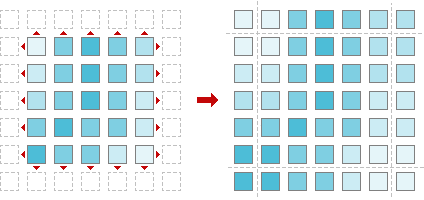
\includegraphics[height=5cm]{img/extendImg.png}
\caption{图像扩展}
\label{fig:imgExt}
\end{figure}
因此,在对图像进行中值滤波之前,先对图片进行扩展,代码实现如下所示:
\begin{lstlisting}
//   Allocate memory for signal extension
	element* extension = new element[(N + 2) * (M + 2)];
	//   Check memory allocation
	if (!extension)
		return;
	//   Create image extension
	for (int i = 0; i < M; ++i)
	{
		memcpy(extension + (N + 2) * (i + 1) + 1, image + N * i, N * sizeof(element));
		extension[(N + 2) * (i + 1)] = image[N * i];
		extension[(N + 2) * (i + 2) - 1] = image[N * (i + 1) - 1];
	}
	//   Fill first line of image extension
	memcpy(extension, extension + N + 2, (N + 2) * sizeof(element));
	//   Fill last line of image extension
	memcpy(extension + (N + 2) * (M + 1), extension + (N + 2) * M, (N + 2) * sizeof(element));
	//   Call median filter implementation
\end{lstlisting}
接下来第二步就是取出窗口中的元素,保存在数组\lstinline{window[]}中。
\begin{lstlisting}
			//   Pick up window elements
			int k = 0;
			element window[9];
			for (int j = m - 1; j < m + 2; ++j)
				for (int i = n - 1; i < n + 2; ++i)
					window[k++] = image[j * N + i];
\end{lstlisting}

第三步就是把窗口中的元素排序。但是在这里我们将会使用一个代码优化的技巧:由于我们需要的仅仅是中值,所以只需要对一半的元素排序就可以了。

\begin{lstlisting}
//   Order elements (only half of them)
			for (int j = 0; j < 5; ++j)
			{
				//   Find position of minimum element
				int min = j;
				for (int l = j + 1; l < 9; ++l)
					if (window[l] < window[min])
						min = l;
				//   Put found minimum element in its place
				const element temp = window[j];
				window[j] = window[min];
				window[min] = temp;
			}
\end{lstlisting}

最后一步,将得到的中值作为该点像素的灰度值。

\begin{lstlisting}
//   Get result - the middle element
			result[(m - 1) * (N - 2) + n - 1] = window[4];
\end{lstlisting}

上述过程即为中值滤波的完整的处理过程,为了方便使用,我们将上述处理过程写在两个函数中。处理前的扩展函数\lstinline{medianfilter()},负责对图像进行扩展,并将扩展好的图像传递给中值滤波函数,其函数参数为原图像指针\lstinline{image}、结果图像指针\lstinline{result}、图像宽度\lstinline{N}、图像高度\lstinline{M};中值滤波函数\lstinline{\_medianfilter()}的工作就是对扩展好的函数进行滤波处理,其函数参数与\lstinline{medianfilter()}相同。
为了将处理结果与OpenCV中的平滑处理函数\lstinline{medianBlur()}的处理结果做对比,我们将函数\lstinline{medianBlur()}的第三个参数模版核的长度设置为3,即与前面的窗口宽度值保持一致。

\begin{lstlisting}
medianBlur(src, dst, 3);
\end{lstlisting}

\section{实验结果}

下图\ref {fig:previous}为原始图像,该图像具有大量的椒盐噪声。

\begin{figure}[h]
\centering
\begin{varwidth}[t]{\textwidth}
\vspace{0pt}
\centering
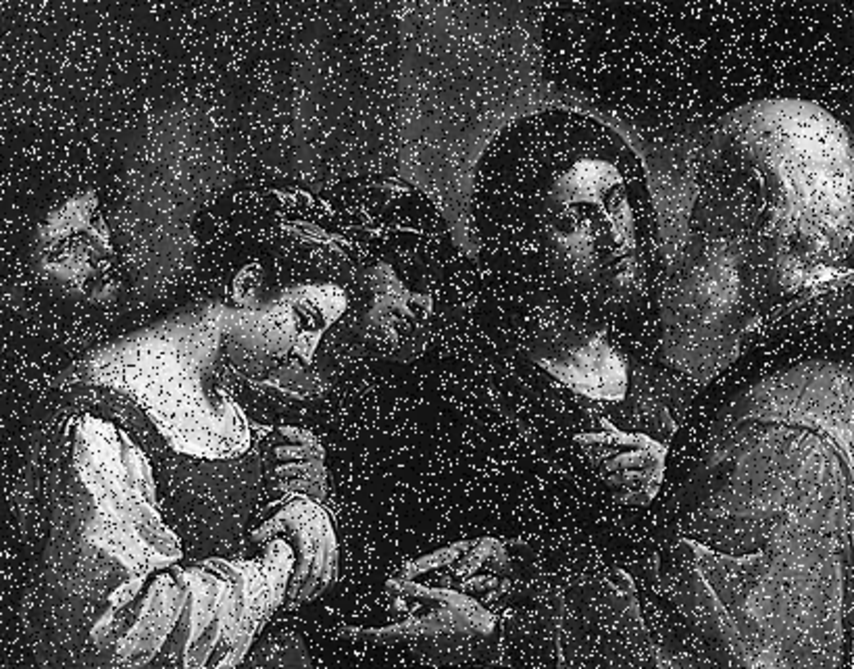
\includegraphics[height=5cm]{img/impulseNoise.pdf}
\caption{椒盐噪声图像}
\label {fig:previous}
\end{varwidth}%
\quad
\begin{varwidth}[t]{\textwidth}
\vspace{0pt}
\centering
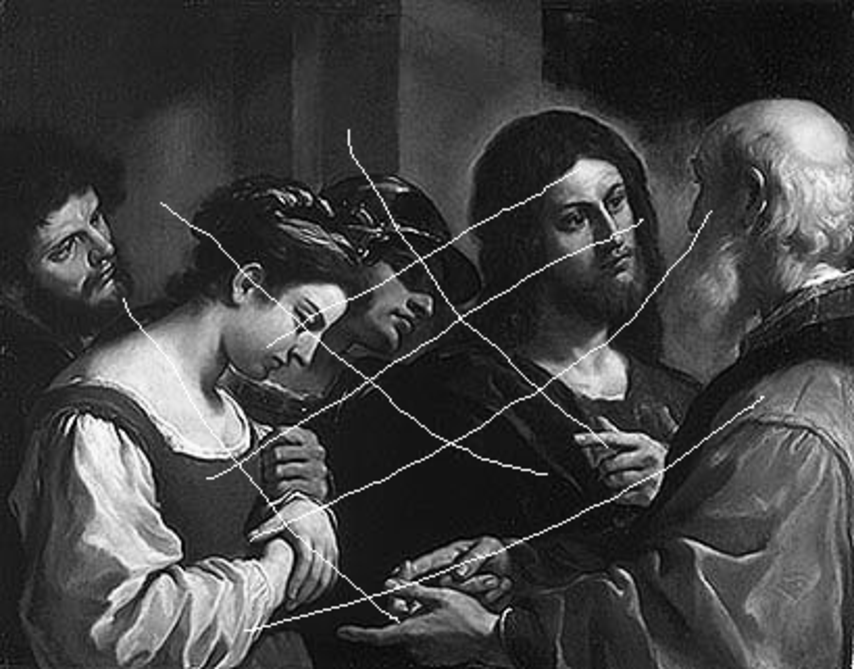
\includegraphics[height=5cm]{img/scratchNoises.pdf}
\caption{充满了抓痕的图像}
\label{fig:scratchedImg}
\end{varwidth}
\end{figure}

下图\ref {fig:firtProc}为不使用OpenCV库函数对图像进行中值滤波的处理结果,模版核的大小为$3\times3$。

\begin{figure}[h]
\centering
\begin{varwidth}[t]{\textwidth}
\vspace{0pt}
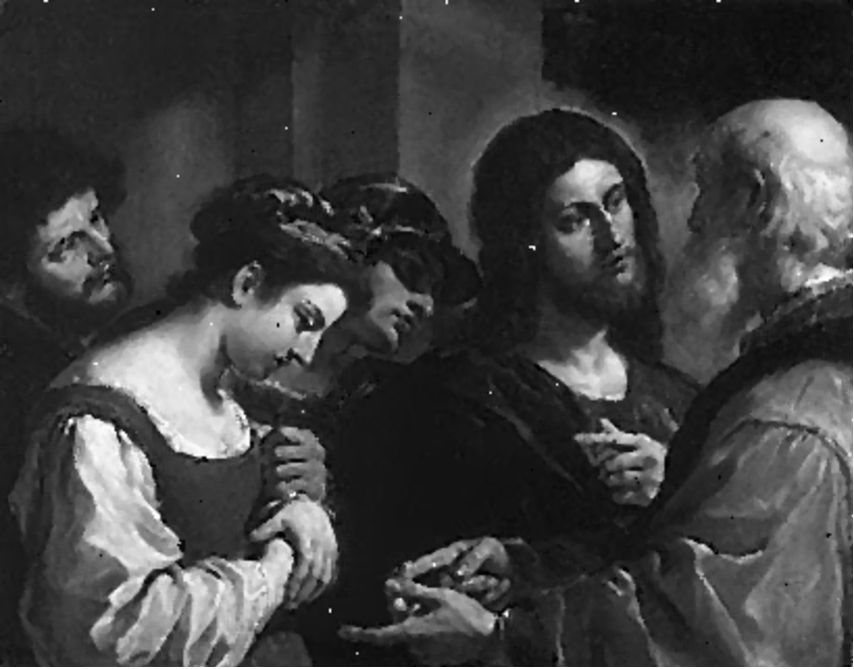
\includegraphics[height=5cm]{img/processedImage1.pdf}
\caption{未使用OpenCV库函数处理的图像}
\label{fig:firtProc}
\end{varwidth}%
\quad
\begin{varwidth}[t]{\textwidth}
\vspace{0pt}
\centering
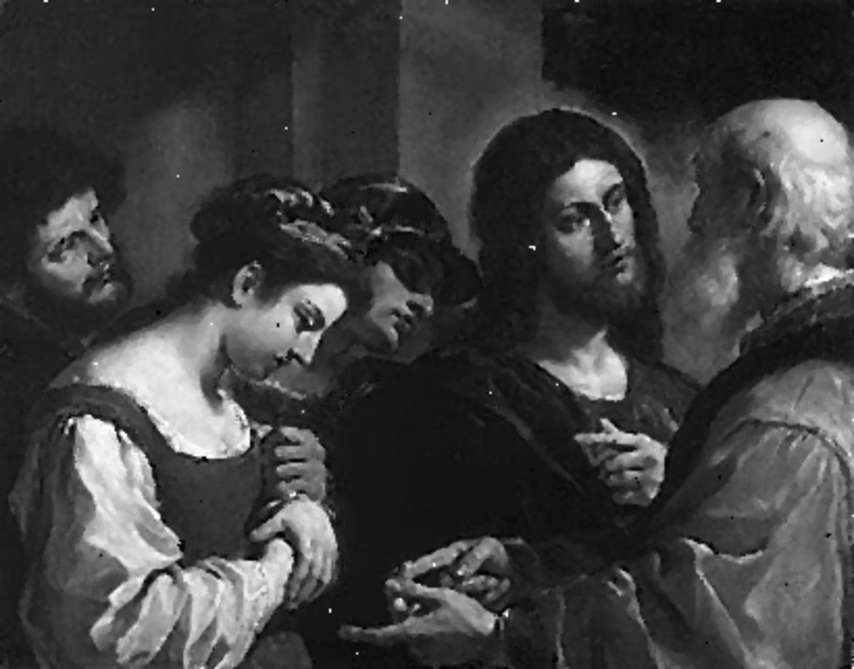
\includegraphics[height=5cm]{img/processedImage2.pdf}
\caption{使用OpenCV库函数处理的图像}
\label{fig:secondProc}
\end{varwidth}
\end{figure}


从图中,不难看出两次处理结果基本相同,差别很小。为了进一步验证上述程序的正确性,我们有对另一种噪声的图像做了相同的处理。

图\ref{fig:scratchedImg}为一张充满了抓痕噪声的图片,同样采用两种方式对其做中值滤波。

结果如下图\ref{fig:thirdProc}和图\ref{fig:forthProc}所示,同样,两次处理结果基本相同。

经过上面两次测试,说明前面编写的程序基本没什么问题,很出色地完成了中值滤波,图像修复得也比较好。

\begin{figure}[H]
\centering
\begin{varwidth}[t]{\textwidth}
\vspace{0pt}
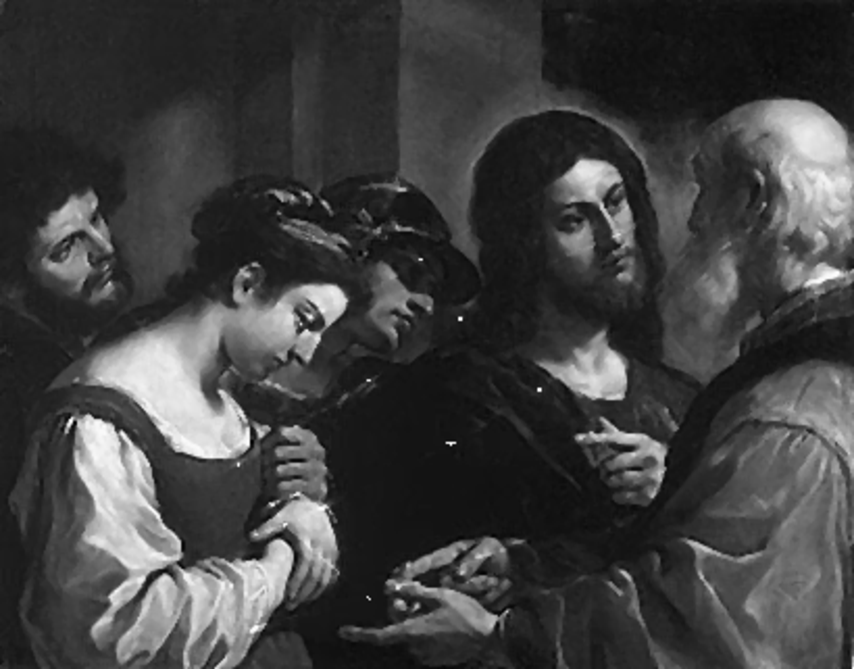
\includegraphics[height=5cm]{img/processedImage3.pdf}
\caption{未使用OpenCV库函数处理的图像}
\label{fig:thirdProc}
\end{varwidth}%
\quad
\begin{varwidth}[t]{\textwidth}
\vspace{0pt}
\centering
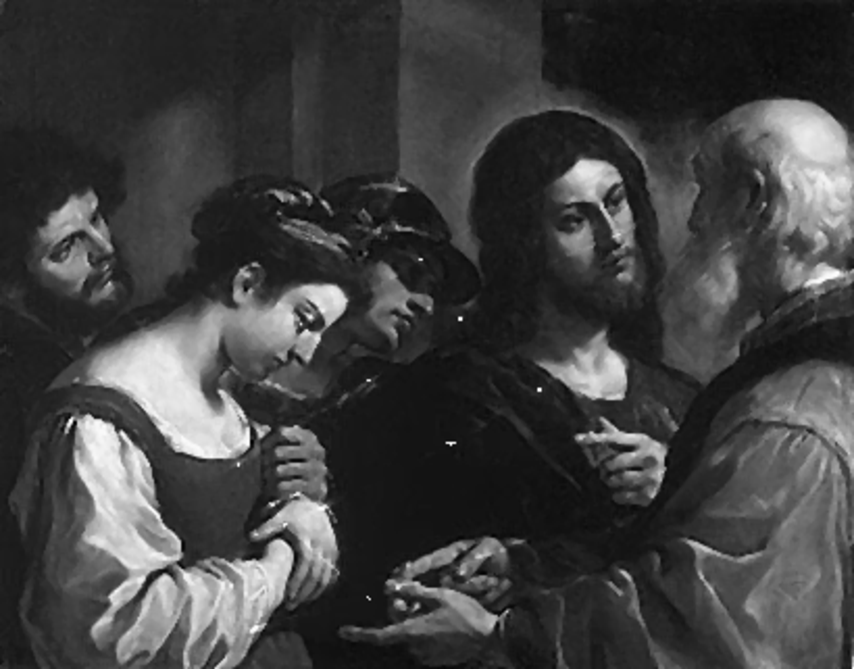
\includegraphics[height=5cm]{img/processedImage4.pdf}
\caption{使用OpenCV库函数处理的图像}
\label{fig:forthProc}
\end{varwidth}
\end{figure}


\section{实验总结}

本次实验主要是为了帮助理解并掌握图像平滑的基本理论和常用方法。为了进一步学习图像平滑的常用方法,特以中值滤波为例,使用C++编程来实现图像的滤波。为了验证程序的正确性,还使用OpenCV的库函数进行同样的操作,并将二者的结果进行对比。

在此次实验中,我不仅学会了如何编程实现中值滤波,掌握了中值滤波的方法,而且我还学会了如何在OpenCV中加载图像、显示图像、保存图像以及调用滤波函数来对图像进行处理。

\end{document}
